\documentclass[conference]{IEEEtran}
\IEEEoverridecommandlockouts%The preceding line is only needed to identify funding in the first footnote. If that is unneeded, please comment it out.

\usepackage[utf8]{inputenc}
\usepackage{cite}
\usepackage{amsmath,amssymb,amsfonts}
\usepackage{algorithmic}
\usepackage{graphicx}
\usepackage{textcomp}
\usepackage{xcolor}
\usepackage{lipsum}


\def\BibTeX{{\rm B\kern-.05em{\sc i\kern-.025em b}\kern-.08em
    T\kern-.1667em\lower.7ex\hbox{E}\kern-.125emX}}

%Para justificar sin cortar palabras
\tolerance=1
\emergencystretch=\maxdimen
\hyphenpenalty=10000
\hbadness=10000

%-------------------------------------------------------------------------------
%	BEGIN DOCUMENT
%-------------------------------------------------------------------------------
\begin{document}

%-------------------------------------------------------------------------------
%	DOCUMENT INFORMATION
%-------------------------------------------------------------------------------
\title{Dithering\\
%{\footnotesize \textsuperscript{*}Note: Sub-titles are not captured in Xplore and should not be used}
%\thanks{Identify applicable funding agency here. If none, delete this.}
}


%-------------------------------------------------------------------------------
%	AUTHORS
%-------------------------------------------------------------------------------
\author{
\IEEEauthorblockN{Daniel Torres Robledo}
\IEEEauthorblockA{\textit{shadow.cat6333@gmail.com}}
\and
\IEEEauthorblockN{Andrés}
\IEEEauthorblockA{\textit{correo@gmail.com}}

}

\maketitle


%-------------------------------------------------------------------------------
%	ABSTRACT
%-------------------------------------------------------------------------------
\begin{abstract}
This document is a model and instructions for \LaTeX.
This and the IEEEtran.cls file define the components of your paper [title, text, heads, etc.]. *CRITICAL: Do Not Use Symbols, Special Characters, Footnotes, 
or Math in Paper Title or Abstract.
\end{abstract}

\begin{IEEEkeywords}
component, formatting, style, styling, insert
\end{IEEEkeywords}

%-------------------------------------------------------------------------------
%	INTRODUCTION
%-------------------------------------------------------------------------------
\section{Introducción}
This document is a model and instructions for \LaTeX.
Please observe the conference page limits.

Prueba \cite{b1}.


%-------------------------------------------------------------------------------
%	SECTION 1
%-------------------------------------------------------------------------------
\section{\textit{Dithering}}
\textcolor{violet}{\lipsum[3]}

%-------------------------------------------------------------------------------
\subsection{Ventajas}
\textcolor{violet}{\lipsum[3]}

%-------------------------------------------------------------------------------
\subsection{Desventajas}
\textcolor{violet}{\lipsum[3]}


%-------------------------------------------------------------------------------
%	SECTION 2
%-------------------------------------------------------------------------------
\section{Implementación}
\textcolor{violet}{\lipsum[3]}

\begin{figure}[htbp]
\centerline{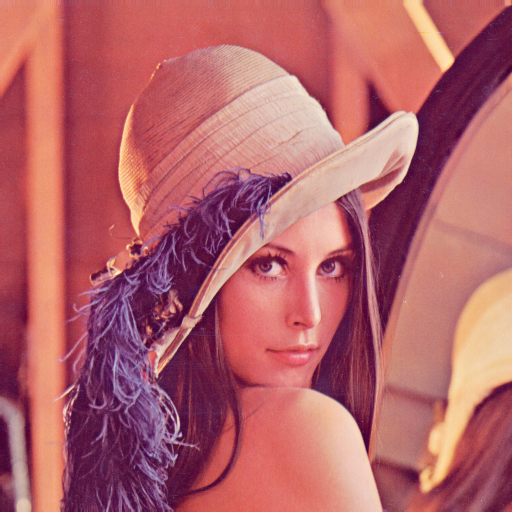
\includegraphics[width=60mm]{code/lena}}
\caption{Example of a figure caption.}
\label{original}
\end{figure}

%-------------------------------------------------------------------------------
\subsection{\textit{Random Dithering}}
\textcolor{violet}{\lipsum[3]}

%-------------------------------------------------------------------------------
\subsection{\textit{Ordered Dithering}}
\textcolor{violet}{\lipsum[3]}

%-------------------------------------------------------------------------------
\subsection{\textit{Random Dithering}}
\textcolor{violet}{\lipsum[3]}








%-------------------------------------------------------------------------------
%	BIBLIOGRAPHY
%-------------------------------------------------------------------------------
\begin{thebibliography}{00}
\bibitem{b1} Team Veryovka-Buchanan, \textit{Developed Algorithms}. Avalible at \textit{https://www.visgraf.impa.br/Courses/ip00/proj/Dithering1/\\algoritmos\_desenvolvidos.htm}. [Accessed Agosto 25, 2019]

\bibitem{b2} Tanner Helland, \textit{Image Dithering: Eleven Algorithms and Source Code}. Avalible at \textit{http://www.tannerhelland.com/4660/dithering-eleven-algorithms-source-code}. [Accessed Agosto 25, 2019]

\bibitem{b3} Ordered Dithering. [Online]. Avalible at \textit{https://en.wikipedia.org/wiki/Ordered\_dithering}. [Accessed Agosto 25, 2019]
\end{thebibliography}

%\vspace{12pt}
%\color{red}
%IEEE conference templates contain guidance text for composing and formatting conference papers. Please ensure that all template text is removed from your conference paper prior to submission to the conference. Failure to remove the template text from your paper may result in your paper not being published.

%-------------------------------------------------------------------------------
%	END DOCUMENT
%-------------------------------------------------------------------------------
\end{document}